\section{実験}
\subsection{実験器具}
\subsubsection{把持対象物}
把持対象物を\refig{obj}に示す.フォースゲージ(\refig{force_gauge})で引っ張ることができるようにそれぞれフックが取り付けられている.

\begin{figure}[h]
\centering
\subfloat[球]{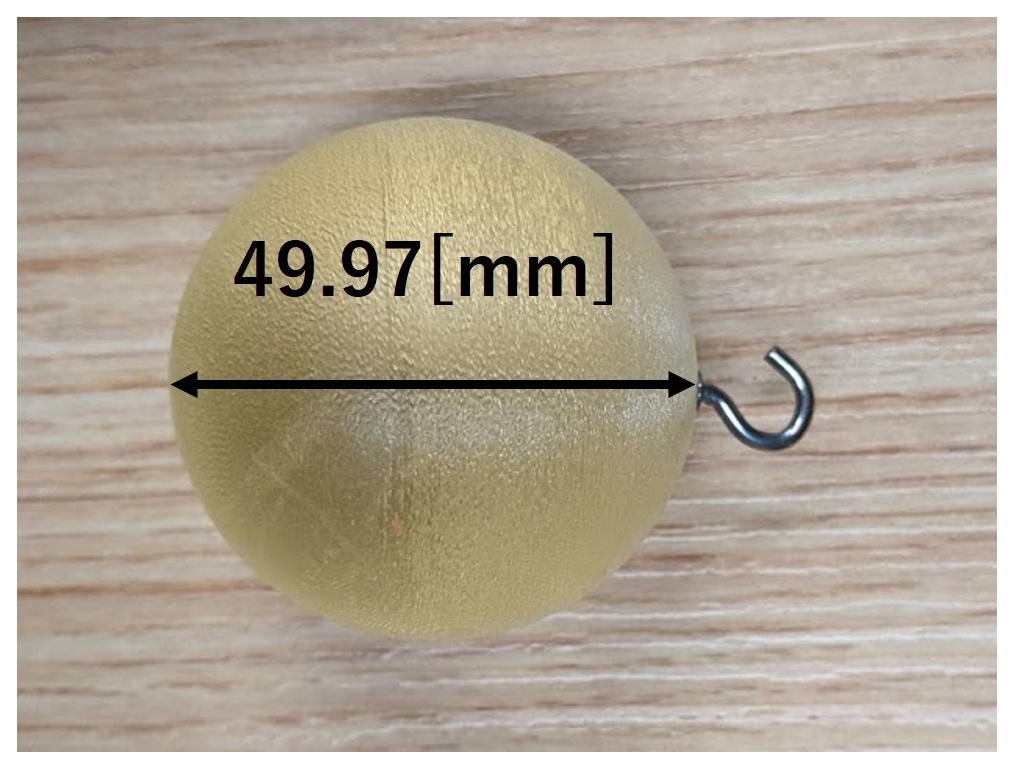
\includegraphics[scale=0.4]{../fig/eps/ball.eps}}
\hspace{7mm}
\\
\subfloat[円筒]{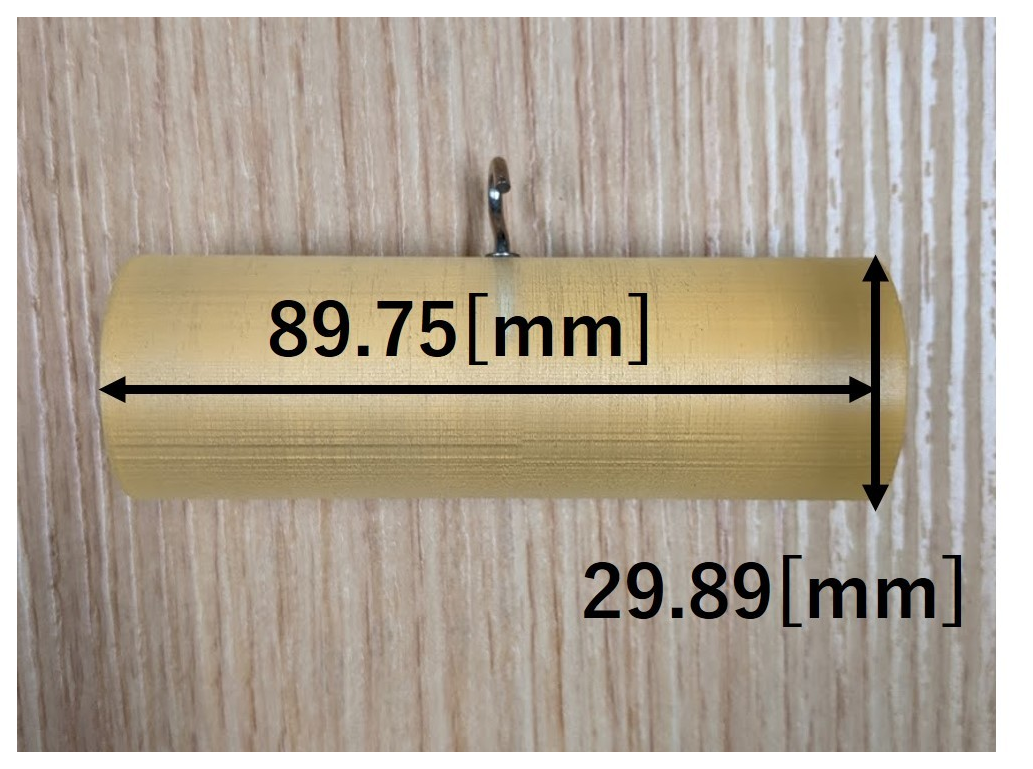
\includegraphics[scale=0.4]{../fig/eps/pole.eps}}
\hspace{7mm}
\subfloat[ボトル]{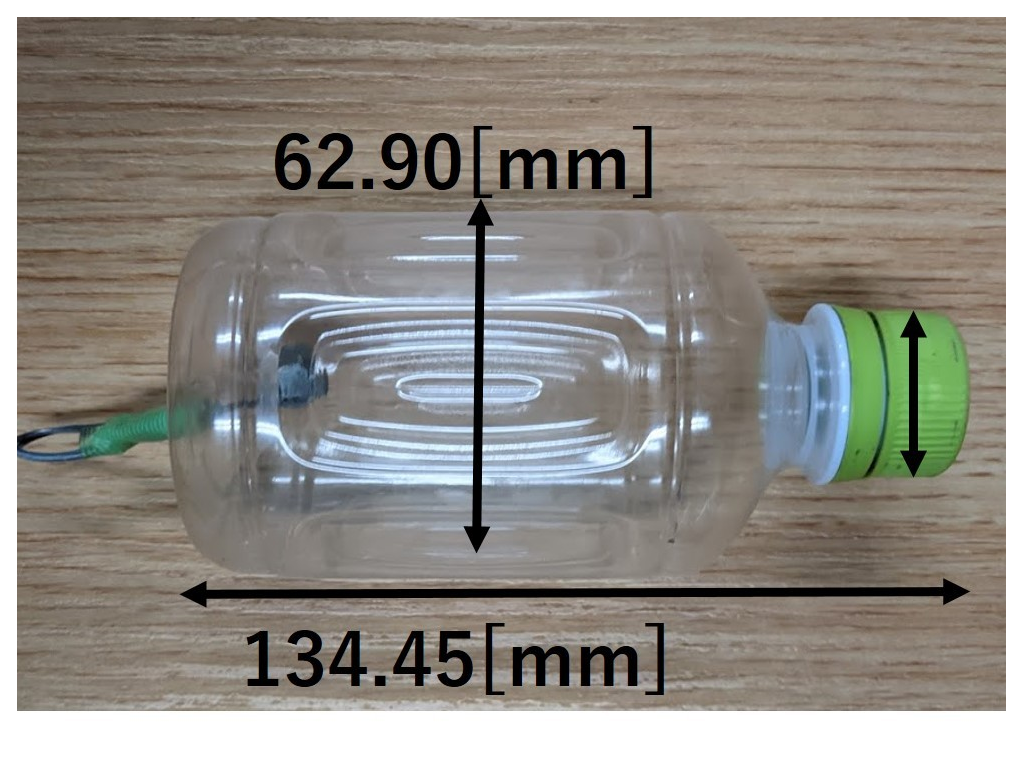
\includegraphics[scale=0.4]{../fig/eps/bottle.eps}}
\hspace{7mm}
\caption{把持対象物}
\label{fig::obj}
\end{figure}

\begin{figure}[h]
 \begin{center}
  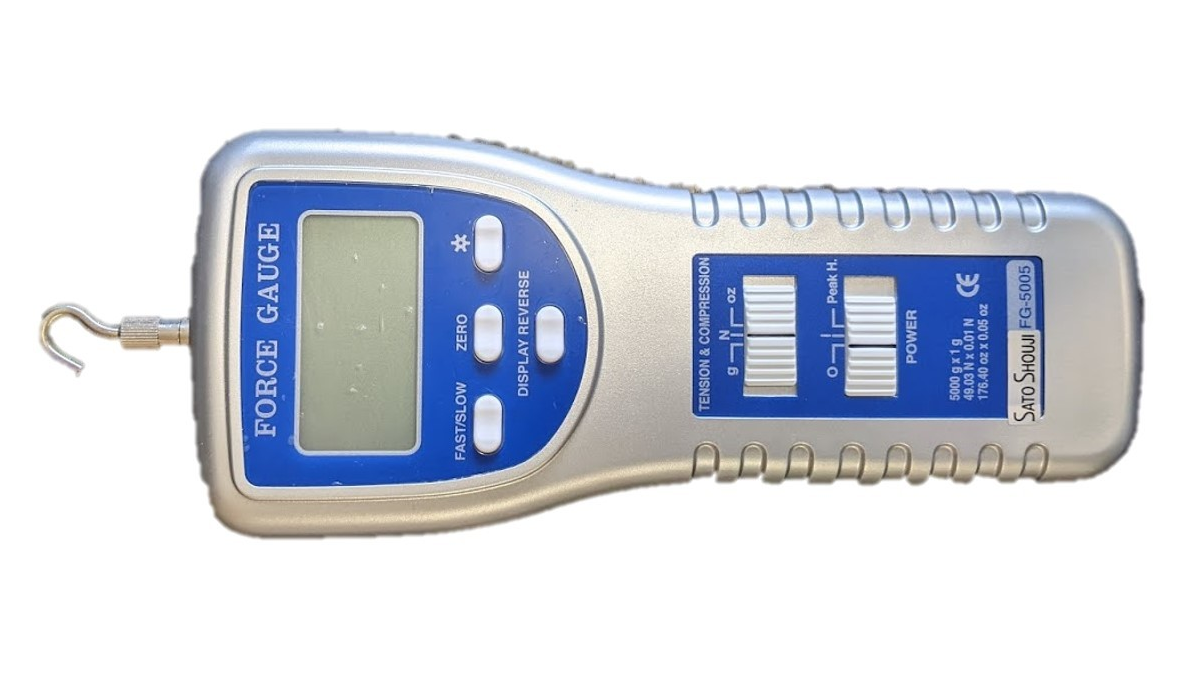
\includegraphics[scale=0.4]{../fig/eps/force_gauge.eps}
 \caption{フォースゲージ}
  \label{fig::force_gauge}
 \end{center}
\end{figure}
\newpage

\subsubsection{センサ使用回路}
イナストマーで力計測をするための専用ソフトウェアである.\refig{ina_kairo}に示す専用回路をPCとUSB接続して用いる.イナストマー購入時に付属される.


\subsubsection{産業用ロボット}
本実験で使用した産業用ロボット(株式会社デンソー製VS087)を\refig{robo}に示す.


\begin{figure}[h]
 \begin{center}
  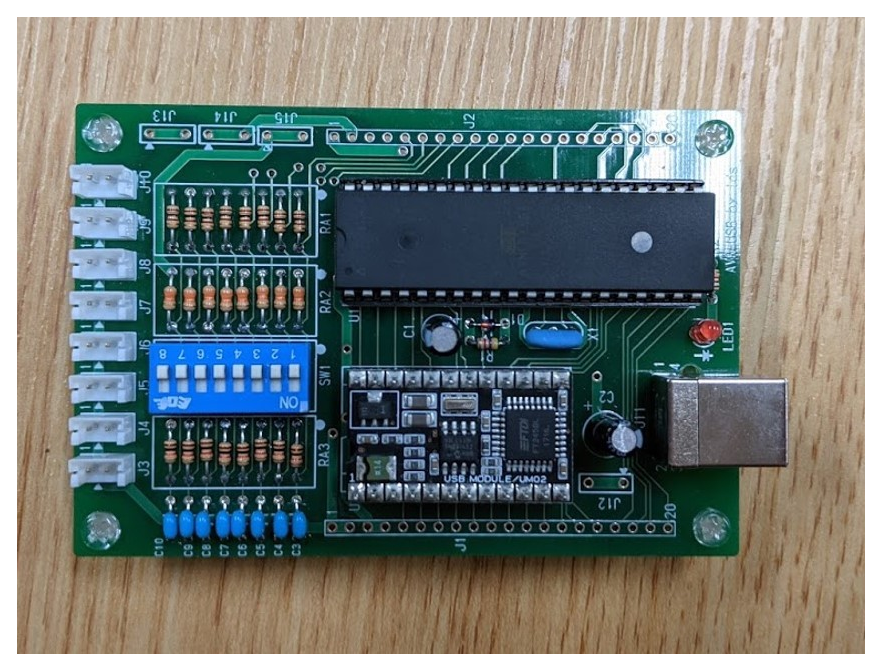
\includegraphics[scale=0.5]{../fig/eps/ina_kairo.eps}
 \caption{専用回路}
  \label{fig::ina_kairo}
 \end{center}
\end{figure}

\begin{figure}[h]
 \begin{center}
  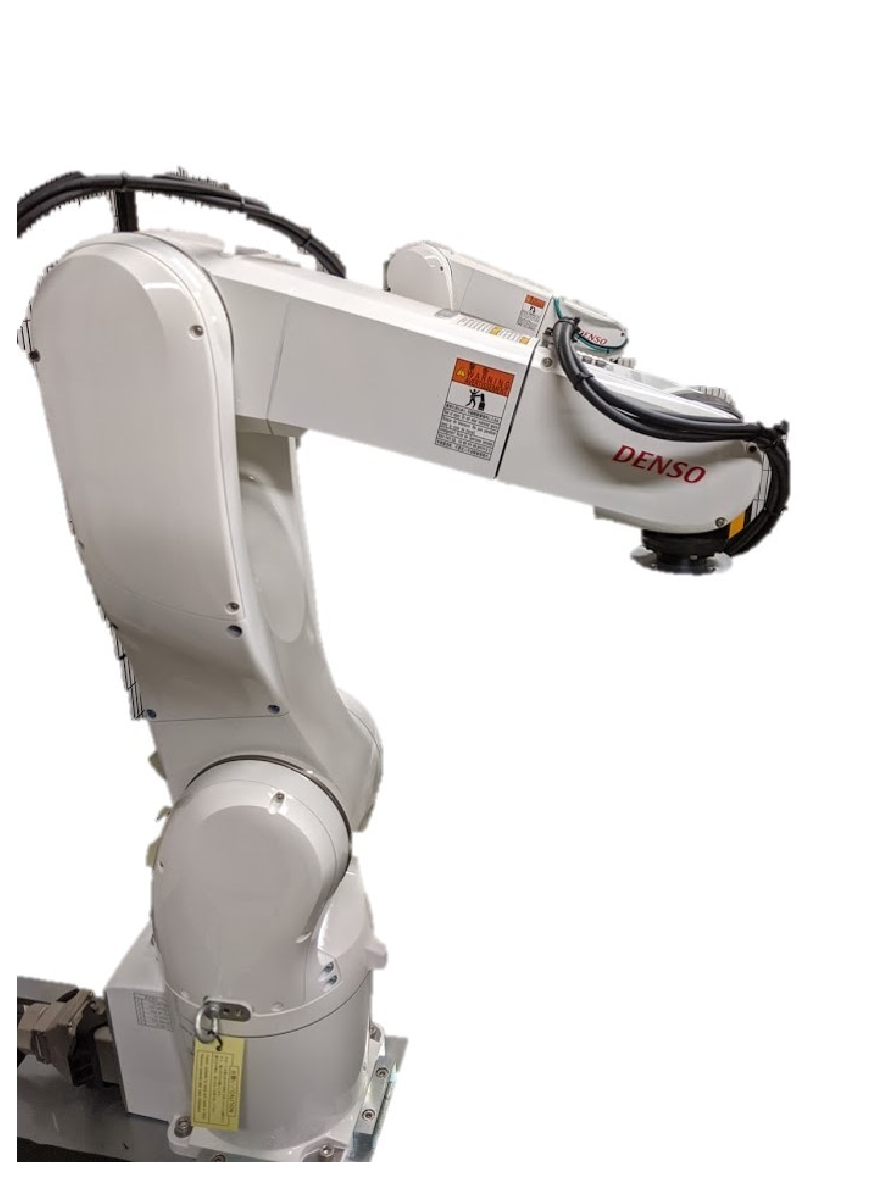
\includegraphics[scale=0.5]{../fig/eps/robo.eps}
 \caption{産業用ロボット}
  \label{fig::robo}
 \end{center}
\end{figure}

\newpage

\subsection{把持実験}
\subsubsection{基礎実験}
力覚センサを組み込んだ通常指及び半球型指を用いて5.0秒間把持対象物を把持したときのセンサの応答を検証した.把持の様子を\refig{grasp1_2}に示す.このときのグリッパの把持力を15.0[N]とした.通常指の結果を\refig{e0_sf},半球型指の結果を\refig{e0_sm}に示す.この実験から両指で把持時に荷重を検出し非把持時には荷重を検出しないことがわかる.

\subsubsection{荷重実験}
力覚センサを組み込んだ通常指及び半球型指を用いて各把持対象物を把持し,グリッパの把持力を15.0[N]から30.0[N]まで増加させた時の力覚センサの応答を計測した.通常指の結果を\refig{result_e2_sf},半球型指の結果を\refig{result_e2_sm}に示す.この実験の結果より把持力の増加に伴い荷重の増加を検出できることが見出された.

\subsubsection{引張実験}
荷重実験と同様に把持しグリッパの把持力を増加させた時に,それぞれの把持力で把持した対象物を鉛直下向きにフォースゲージで引っ張り把持対象物が動いたときの静止摩擦力を計測した.荷重実験と同様にグリッパの把持力を増加させ繰り返した.把持対象物ごとの通常指及び半球型指の結果を\refig{result_e3}を示す.この実験の結果より通常指の方が半球型指に比べて静止摩擦力が大きいことが分かる.
\begin{figure}[htbp]
\centering
\subfloat[通常指]{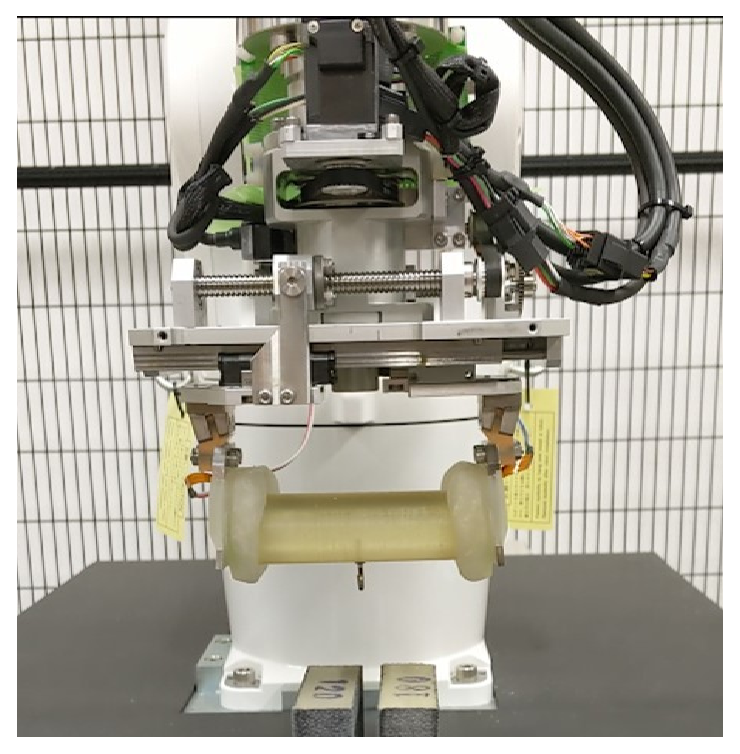
\includegraphics[scale=0.4]{../fig/eps/grasp1.eps}}
\hspace{5mm}
\subfloat[半球型指]{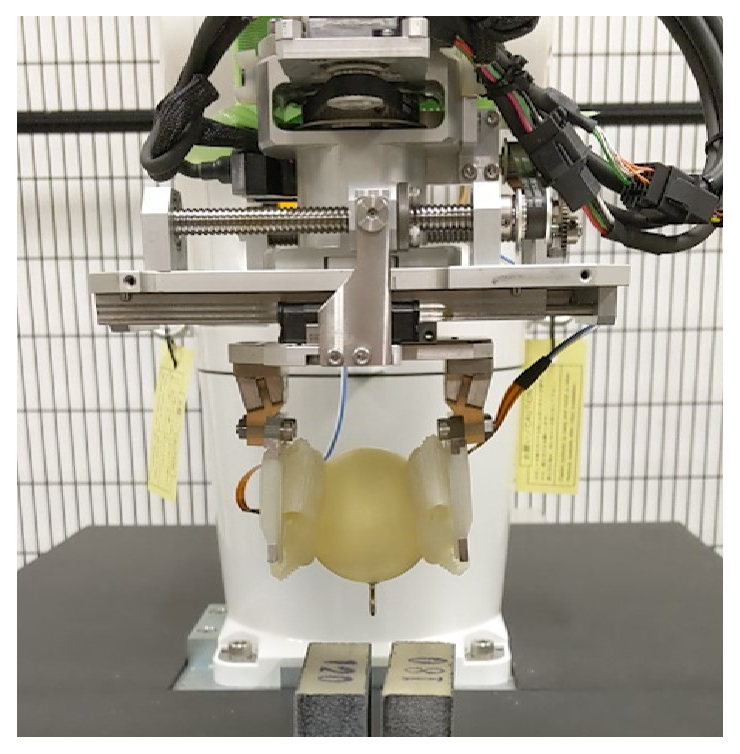
\includegraphics[scale=0.4]{../fig/eps/grasp2.eps}}
\hspace{5mm}\\
\caption{把持の様子}
\label{fig::grasp1_2}
\end{figure}



\begin{figure}[htbp]
\centering
\subfloat[球]{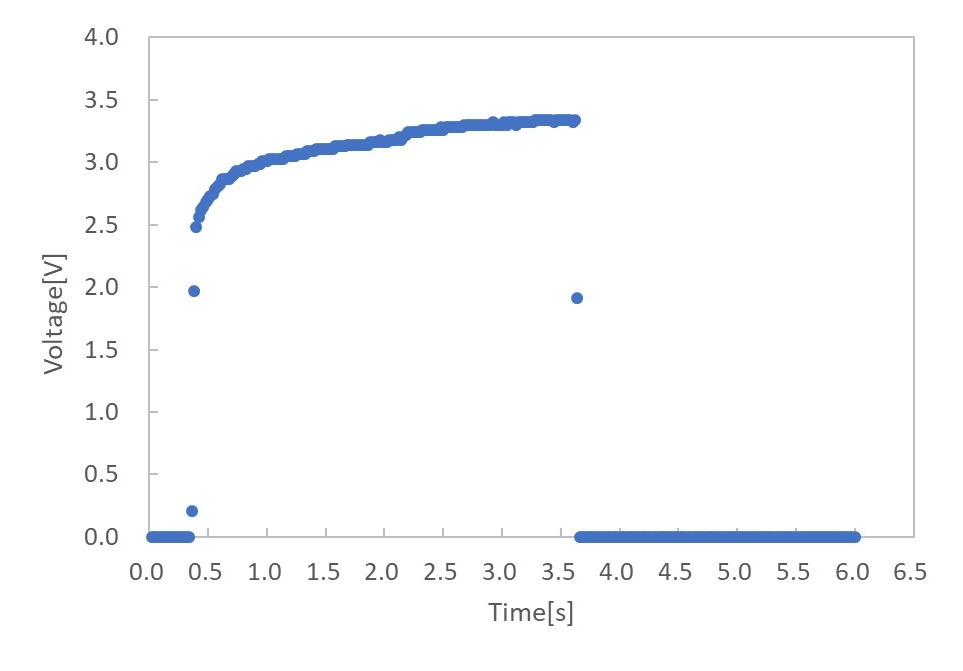
\includegraphics[scale=0.65]{../fig/eps/e0_sf_ball.eps}}
\hspace{5mm}\\
\subfloat[円筒]{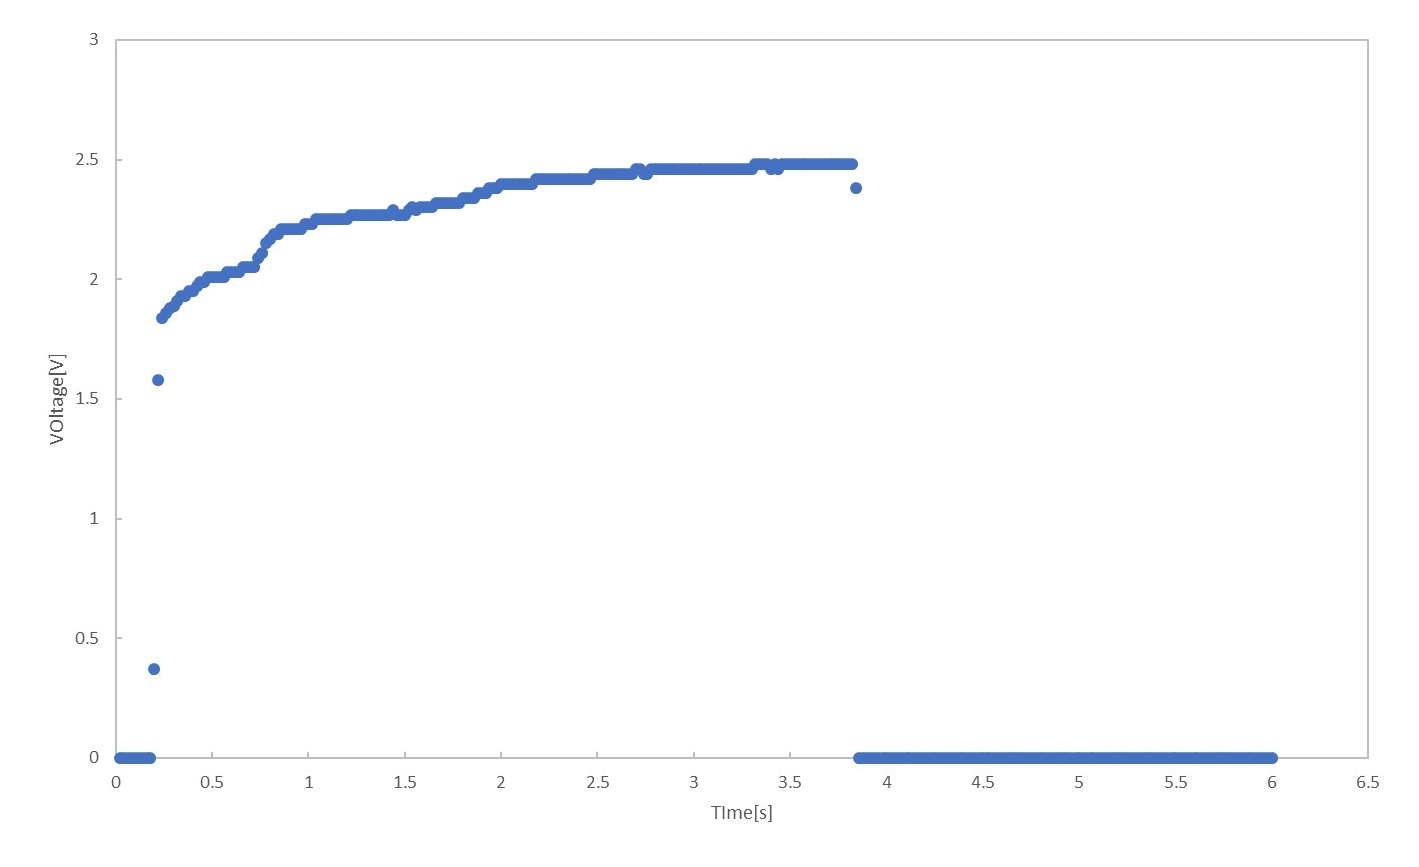
\includegraphics[scale=0.65]{../fig/eps/e0_sf_pole.eps}}
\hspace{5mm}\\
\subfloat[ボトル]{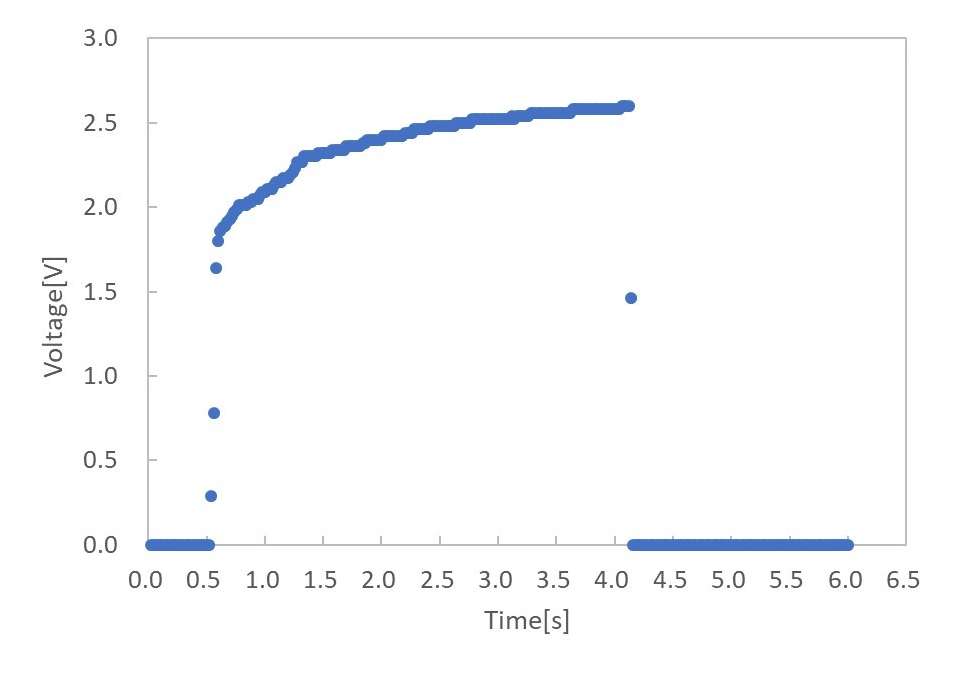
\includegraphics[scale=0.65]{../fig/eps/e0_sf_bottle.eps}}
\hspace{5mm}\\
\caption{把持実験結果(通常指)}
\label{fig::e0_sf}
\end{figure}

\clearpage

\begin{figure}[htbp]
\centering
\subfloat[球]{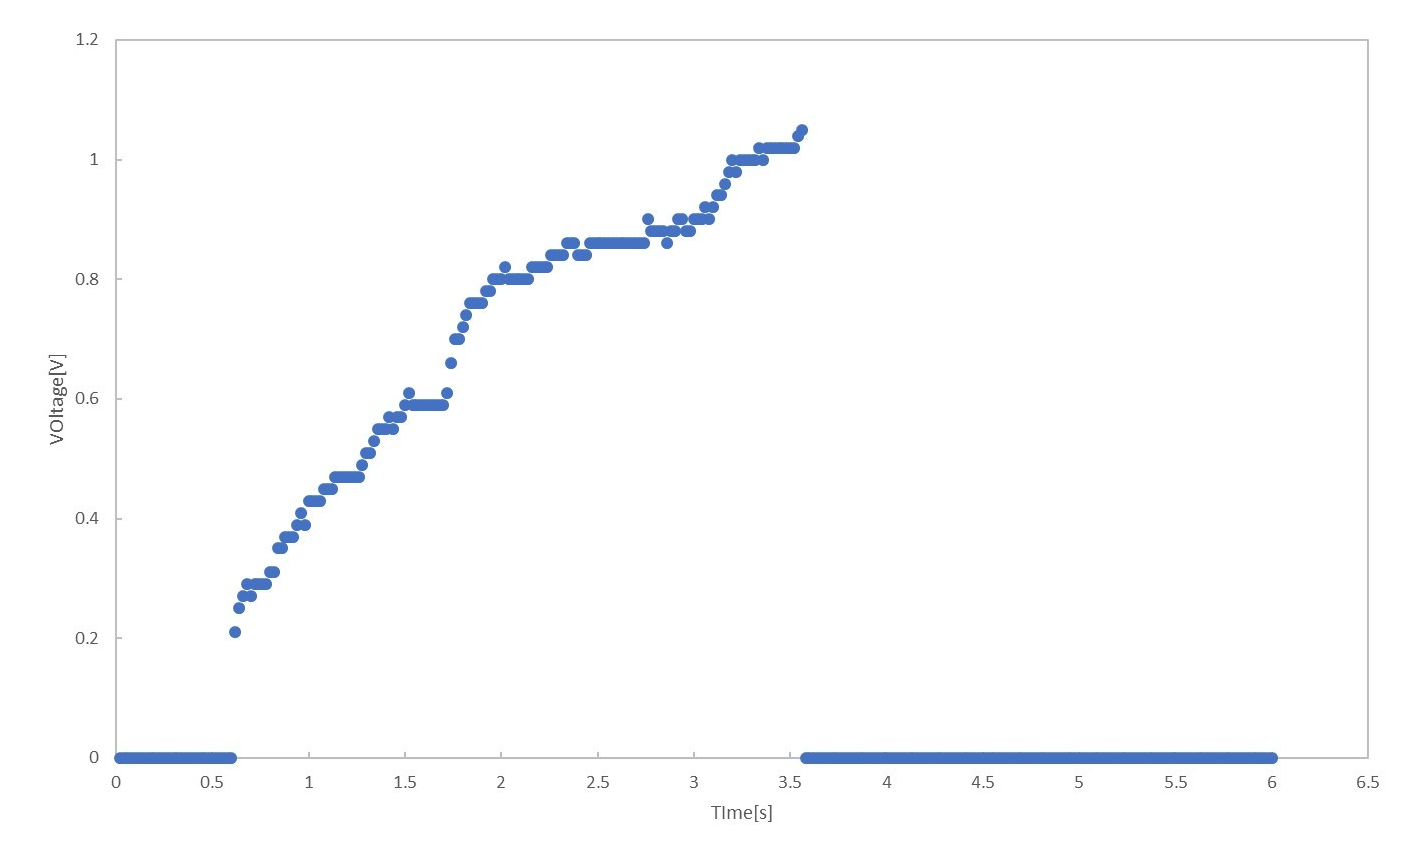
\includegraphics[scale=0.65]{../fig/eps/e0_sm_ball.eps}}
\hspace{5mm}\\
\subfloat[円筒]{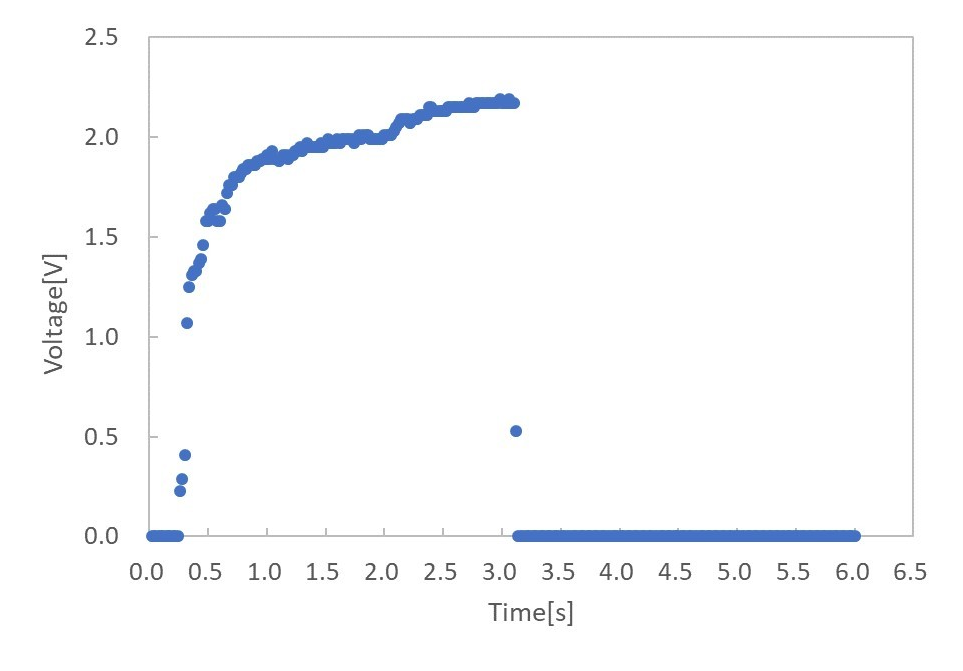
\includegraphics[scale=0.65]{../fig/eps/e0_sm_pole.eps}}
\hspace{5mm}\\
\subfloat[ボトル]{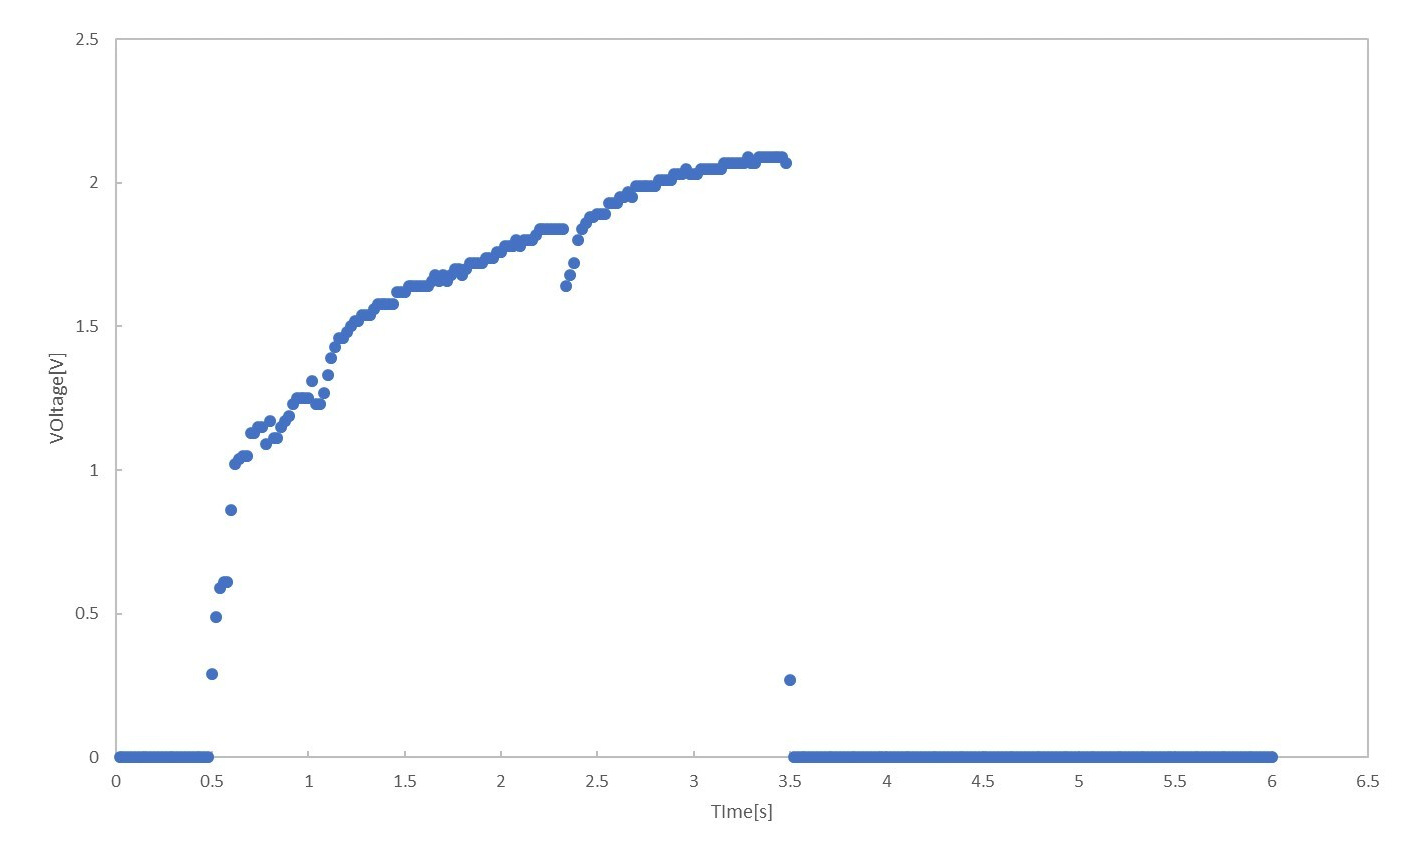
\includegraphics[scale=0.65]{../fig/eps/e0_sm_bottle.eps}}
\hspace{5mm}
\caption{把持実験結果(半球型指)}
\label{fig::e0_sm}
\end{figure}

\clearpage



\begin{figure}[htbp]
\centering
\subfloat[球]{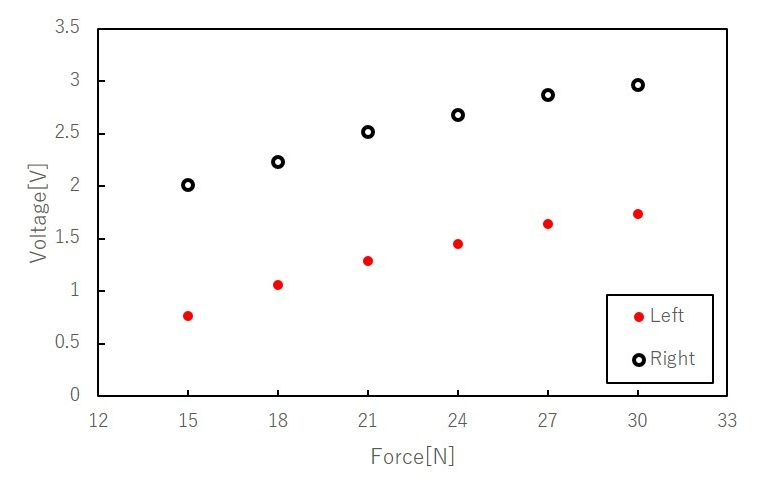
\includegraphics[scale=0.7]{../fig/eps/e2_sf_ball.eps}}
\hspace{5mm}\\
\subfloat[円筒]{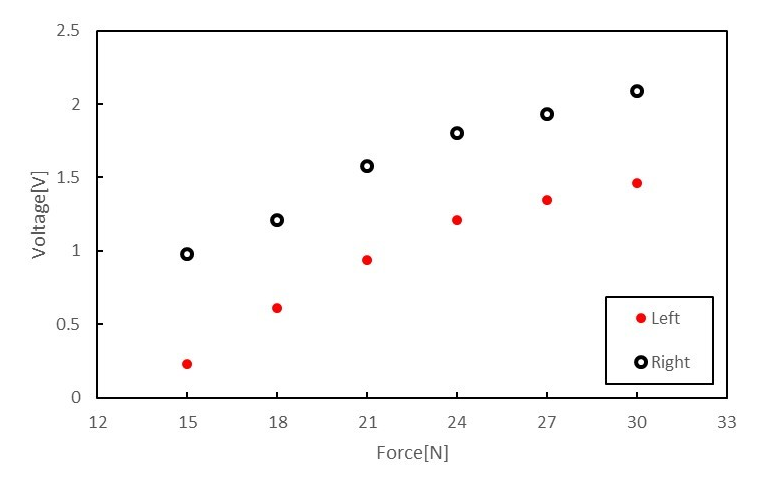
\includegraphics[scale=0.7]{../fig/eps/e2_sf_pole.eps}}
\hspace{5mm}\\
\subfloat[ボトル]{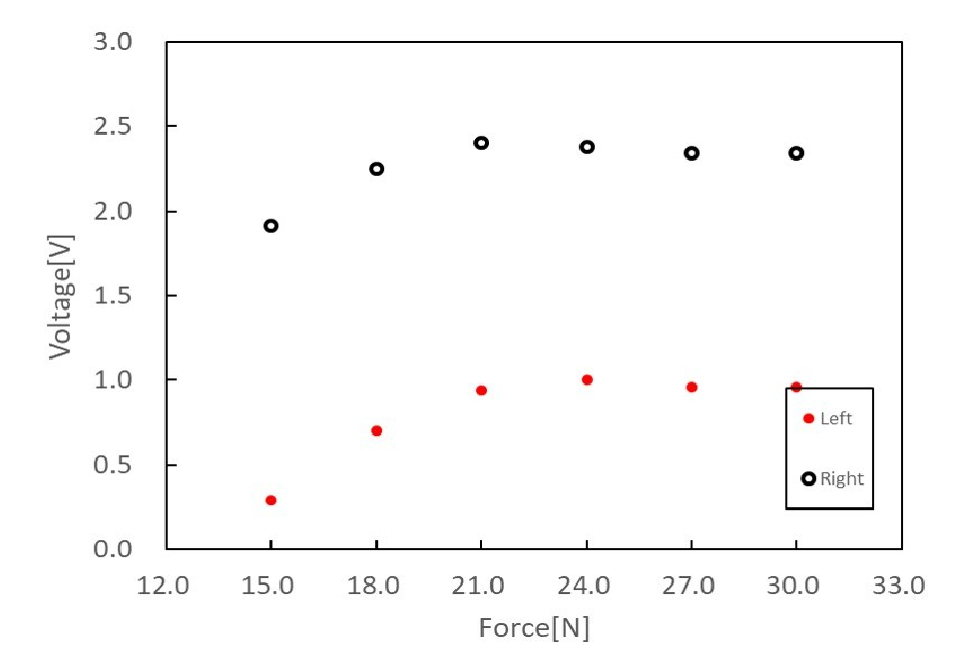
\includegraphics[scale=0.7]{../fig/eps/e2_sf_bottle.eps}}
\hspace{5mm}\\
\caption{荷重実験結果(通常指)}
\label{fig::result_e2_sf}
\end{figure}

\clearpage

\begin{figure}[htbp]
\centering
\subfloat[球]{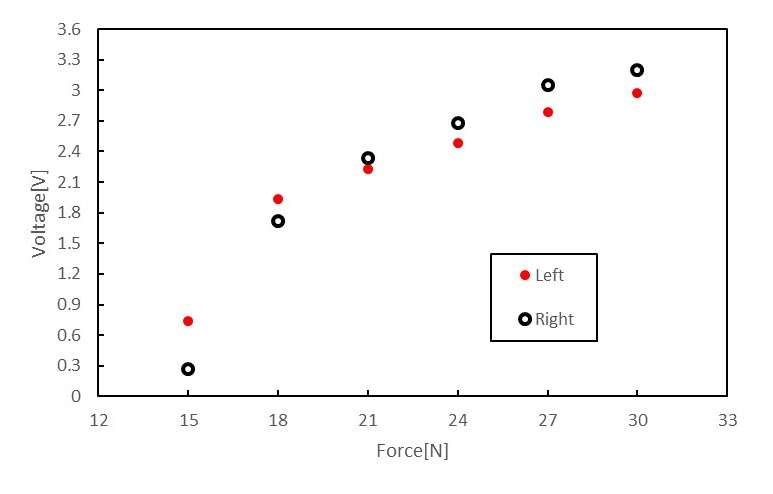
\includegraphics[scale=0.7]{../fig/eps/e2_sm_ball.eps}}
\hspace{5mm}\\
\subfloat[円筒]{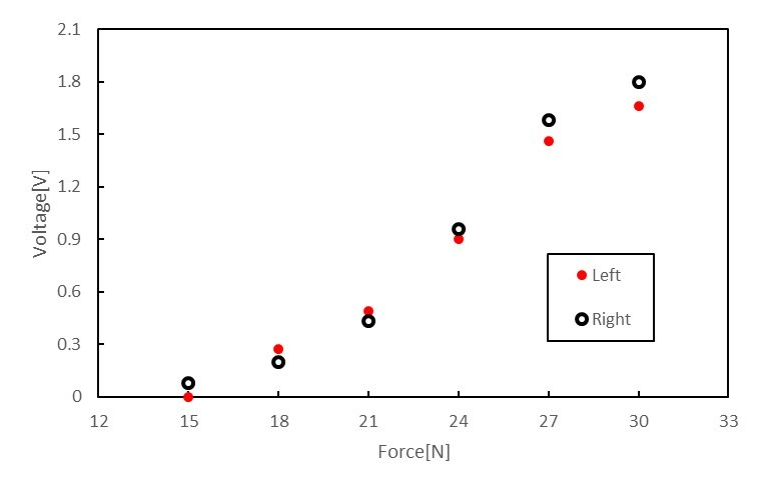
\includegraphics[scale=0.7]{../fig/eps/e2_sm_pole.eps}}
\hspace{5mm}\\
\subfloat[ボトル]{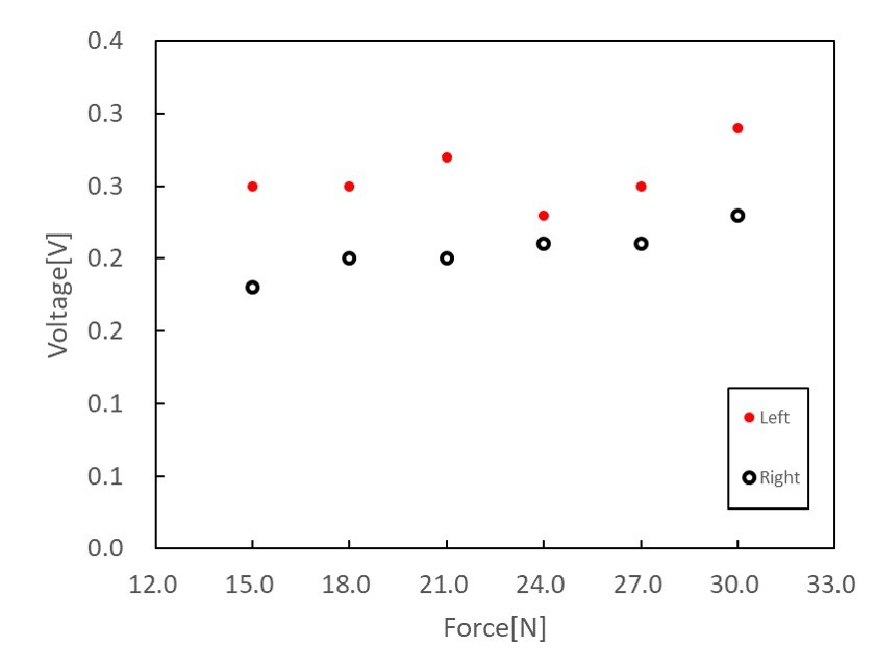
\includegraphics[scale=0.7]{../fig/eps/e2_sm_bottle.eps}}
\hspace{5mm}\\
\caption{荷重実験結果(半球型指)}
\label{fig::result_e2_sm}
\end{figure}

\clearpage

\begin{figure}[htbp]
\centering
\subfloat[球]{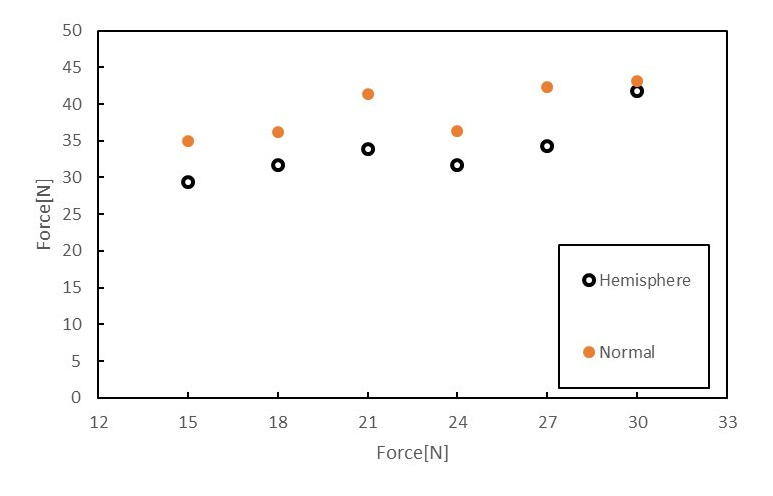
\includegraphics[scale=0.65]{../fig/eps/e3_ball.eps}}
\hspace{5mm}\\
\subfloat[円筒]{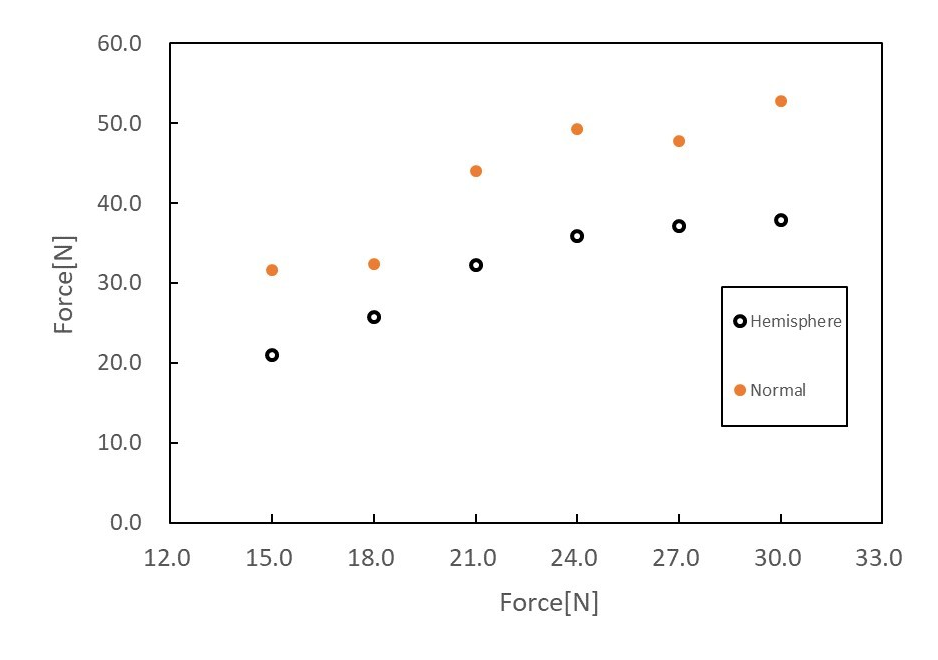
\includegraphics[scale=0.65]{../fig/eps/e3_cylinder.eps}}
\hspace{5mm}\\
\subfloat[ボトル]{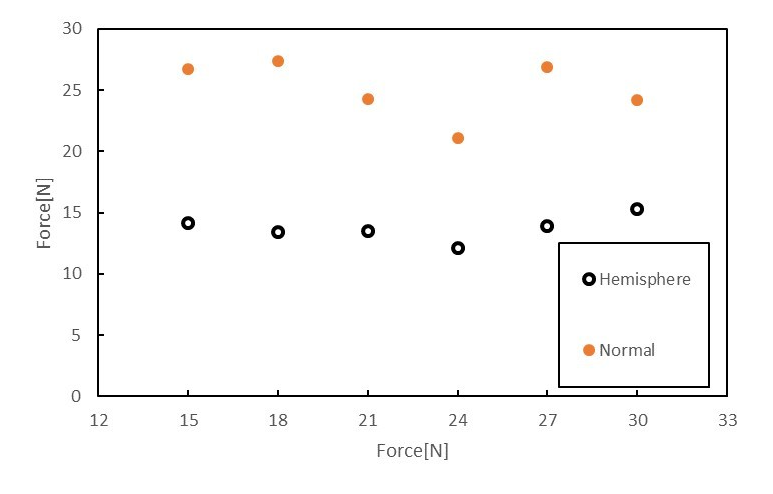
\includegraphics[scale=0.65]{../fig/eps/e3_bottle.eps}}
\hspace{5mm}\\
\caption{引張実験結果}
\label{fig::result_e3}
\end{figure}

\clearpage


